\documentclass[ngerman]{gdb-aufgabenblatt}

\usepackage{graphicx}
\renewcommand{\Aufgabenblatt}{3}
\renewcommand{\Ausgabedatum}{Mi. 12.11.2014}
\renewcommand{\Abgabedatum}{Fr. 28.11.2014}
\renewcommand{\Gruppe}{Schuh, Sibbel, Wille}


\begin{document}

\section{Informationsmodellierung mit dem Entity-Relationship-Modell}

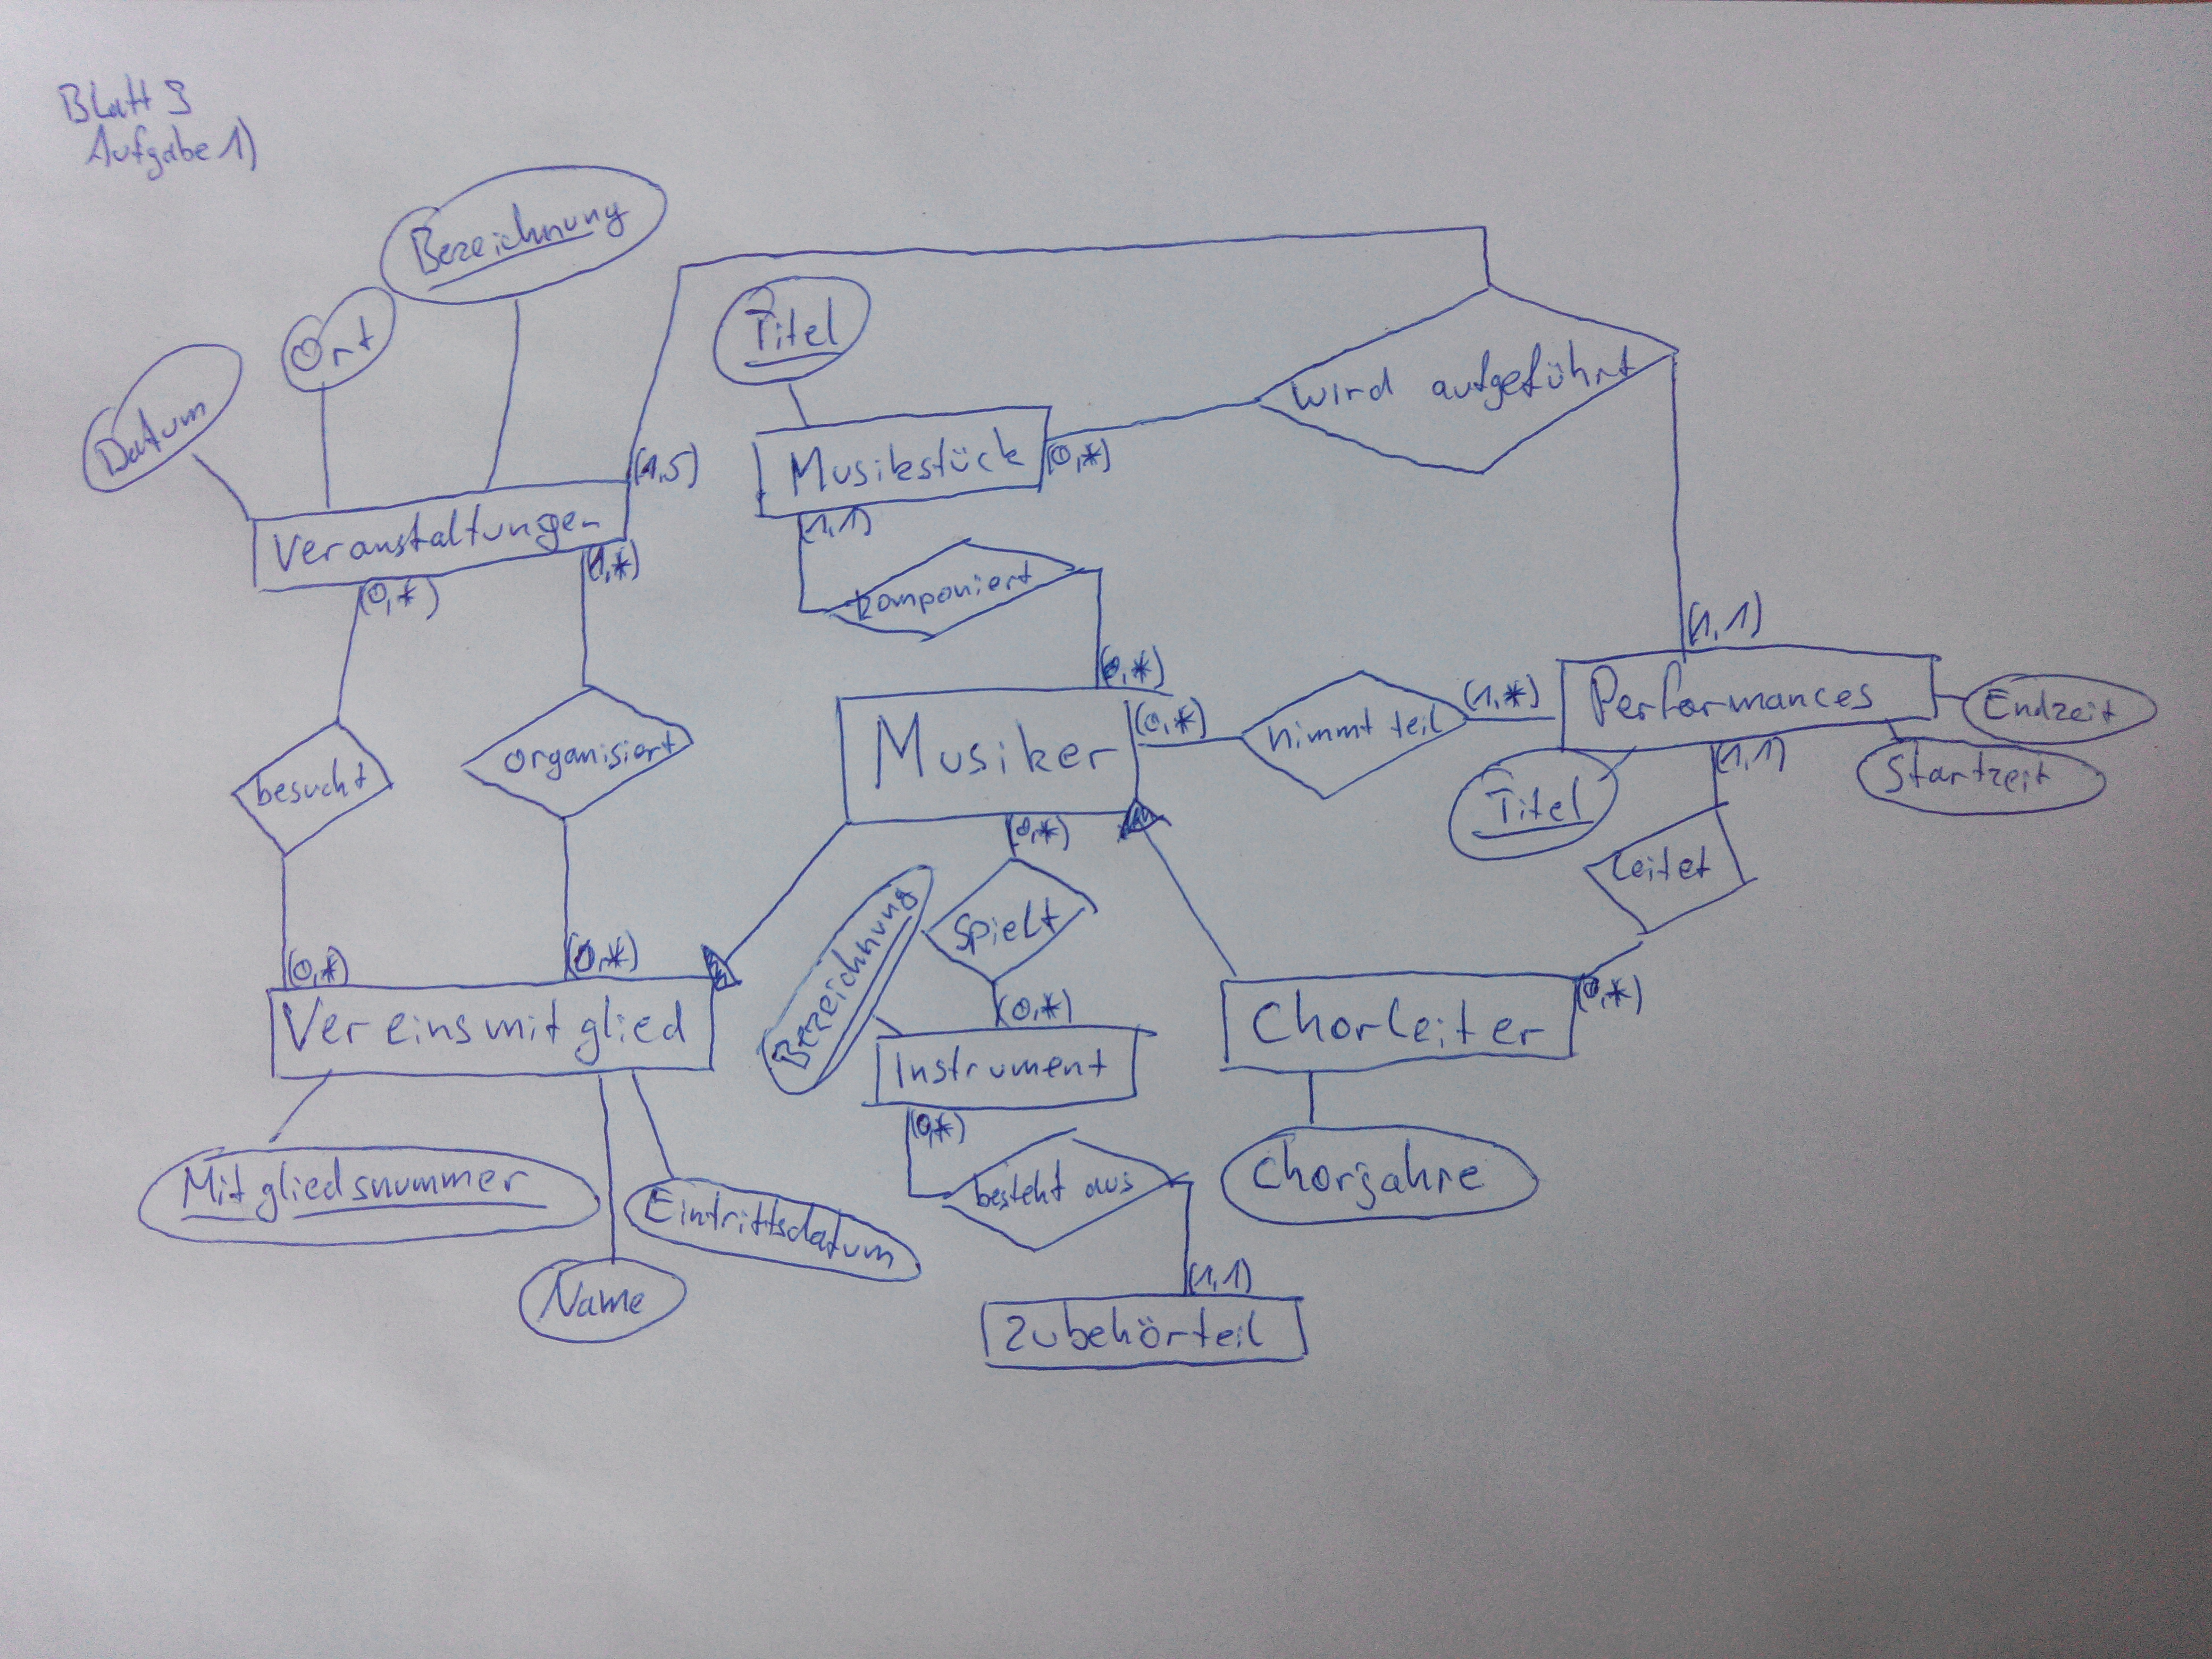
\includegraphics[scale=0.091]{1a.jpg}
\section{Abbildung eines ER-Diagramms auf das relationale
Datenmodell}
\begin{enumerate}
\item[a)]
\begin{RMSchma}
Set(\soliduline{SNr}, Alter,\dashuline{Thema$\rightarrow$Thema.Bez})\\
Werbeset(\soliduline{\dashuline{SNr$\rightarrow$Set.SNr}},Firma)\\
Verkaufsset(\soliduline{\dashuline{SNr$\rightarrow$Set.SNr}},LPreis)\\
Thema(\soliduline{Bez})\\ 
Modell(\soliduline{Name},\soliduline{Datum}, Grad)\\
zugeordnet(\soliduline{\dashuline{Thema$\rightarrow$Thema.Bez, Modellname$\rightarrow$Modell.Name,Modelldatum$\rightarrow$Modell.Datum}})\\
Baustein(\soliduline{Form},Bild,\dashuline{Farbe$\rightarrow$Farbe.RGB})\\
Farbe(\soliduline{RGB},CMYK)\\
enth\"alt(\soliduline{\dashuline{Set$\rightarrow$Set.SNr, Modell$\rightarrow$Modell.Name, Modell$\rightarrow$Modell.Datum, Farbe$\rightarrow$Farbe.RGB,}}\\\dashuline{\soliduline{ Baustein$\rightarrow$Baustein.Form, Teil-Anzahl)}}\\
\end{RMSchma}
\item[b)]
Bei Vererbung werden im Hausklassenmodell Einträge nur in die unterste Klasse geschrieben. Somit sind Abfragen nach Elementen in den Oberklassen aufwändiger.\\
\end{enumerate}
\section{Relationale Algebra und SQL}
\begin{enumerate}
\item[a)]
\begin{enumerate}
\item[i)]
\begin{align*}
&\projektion{Titel}(\selektion{Seitenzahl>200 \land Erscheinungsjahr>1950})\\
&=\{Schall und Wahn, Der Fremde\}
\end{align*}
\item[ii)]
\begin{align*}
&\projektion{Vorname, Nachname} \left( \selektion{Buch=Der Talisman}\left( Person\verbund{Person.PID=Schreibt.Autor}Schreibt \right) \right)\\
&=\{  \}
\end{align*}
\item[iii)]
\begin{align*}
&\projektion{Vorname, Nachname} \left( \selektion{Person \verbund{Lieblingsbuch=Buch}Begutachtet \land Person \verbund{PID=Lektor}Begutachtet}\right)\\
&=\{  \}
\end{align*}
\end{enumerate}
\item[b)]
\begin{enumerate}
\item[i)]
Alle Buchtitel die noch nicht begutachtet wurden.\\
$\{Schall und Wahn, Der Talisman\}$
\item[ii)]
Personen, die ein Buch geschrieben und ein weiteres Buch begutachtet haben.\\
$\{Leo Tolskoi, Fjodor Dostojewski, Albert Camus, William Faulkner,$\\$ Stephen King, Peter Straub, Gabriel Garcia Marquez \}$
\item[iii)]
Vor- und Nachname der Person die ihr eigenes Buch begutachtet haben.\\
$\{ \}$
\end{enumerate}
\item[c)]
\begin{enumerate}
\item[i)]
\begin{verbatim}
SELECT DISTINKT
  Vorname,
  Nachname
FROM 
  Person
WHERE
  Buch.Seitenzahl >= 500
\end{verbatim}
\item[ii)]
\begin{verbatim}
SELECT 
  Titel
FROM 
  Buch
WHERE
  Schreibt.Autor = Begutachtet.lektor
\end{verbatim}
\item[iii)]
\begin{verbatim}
SELECT 
  Vorname, Nachname
FROM 
  Person
WHERE
  Person.PID NOT Gebutachtet.Lektor
\end{verbatim}
\end{enumerate}
\end{enumerate}
\section{Algebraische Optimierung}
\begin{enumerate}
\item[] A1 \\
\begin{tikzpicture}
\node (Buch) {Buch};
\node (selektion1) [above=of Buch] {$\selektion{Seitenzahl>200 \land Verlag = Fischer}$};
\path (selektion1) edge node[smallr,midway,left] {} (Buch);
\node (Person) [right=25mm of selektion1] {Person};
\node (join1) [above=20mm of $(selektion1)!.5!(Person)$] {$\verbund{Buch.Titel=Person.Lieblingsbuch}$};
\path (selektion1) edge node[smallr,near start,above right] {} (join1);
\path (Person) edge node[smalll,near start,above left] {} (join1);
\node (projektion) [above=of join1] {$\projektion{Vorname, Nachname, Titel}$};
\path (join1) edge node[smallr,midway,left] {} (projektion);
\end{tikzpicture}
\clearpage
\item[] A2 \\
\begin{tikzpicture}
\node (Buch) {Buch};
\node (Person) [left=25mm of Buch] {Person};
\node (join1) [above=20mm of $(Buch)!.5!(Person)$] {$\verbund{Buch.Titel=Person.Lieblingsbuch}$};
\node (selektion1) [above=of join1] {$\selektion{Seitenzahl>200 \land Verlag = Fischer}$};
\node (projektion) [above=of selektion1] {$\projektion{Vorname, Nachname, Titel}$};
\node (final) [above=of projektion] {};

\path (Buch) edge node[smallr,near start,above right] {} (join1);
\path (Person) edge node[smalll,near start,above left] {} (join1);
\path (join1) edge node[smallr,near start,above left] {} (selektion1);
\path (selektion1) edge node[smallr,midway,left] {} (projektion);
%\path (projektion) edge node[smallr,midway,left] {$??$ Tupel\\1 Attribut} (final);
\end{tikzpicture}

\item[] A3\\
\begin{tikzpicture}
\node (Buch) {Buch};
\node (selektion1) [above=of Buch] {$\selektion{Seitenzahl>200}$};
\path (selektion1) edge node[smallr,midway,left] {} (Buch);
\node (selektion2) [above=of selektion1] {$\selektion{Verlag = Fischer}$};
\path (selektion2) edge node[smallr,midway,left] {} (selektion1);
\node (join1) [above=20mm of $(selektion2)!.5!(Person)$] {$\verbund{Buch.Titel=Person.Lieblingsbuch}$};
\node (Person) [left=25mm of selektion2] {Person};
\path (join1) edge node[smallr,midway,left] {} (selektion2);
\path (join1) edge node[smalll,near start,above left] {} (Person);
\node (projektion) [above=of join1] {$\projektion{Vorname, Nachname, Titel}$};
\path (join1) edge node[smallr,midway,left] {} (projektion);
\end{tikzpicture}
\end{enumerate}
A1 hat den h\"ochsten Optimierungsgrad, da die Selektion als erstes ausgef\"uhrt wird(Heuristik I) und diese in einem Schritt zusammen gefasst ist(III).

%\begin{align*}
% &\projektion{Rasse, Geschlecht}((Wolf\verbund{Wolf.WID=Haustier.HID} (\selektion{Name=\wert{Hasso}}Haustiere)) \natverbund Person)
%\\  &=\{ \wert{Steppenwolf}, \wert{m} \}
%\end{align*}

%\begin{RMSchma}
%Person(\soliduline{PID}, Name, Vorname)
%
%Haustier(\soliduline{HID}, Name, Rasse, \dashuline{Herrchen $\rightarrow$ Person.PID})
%\end{RMSchma}






\end{document}
